\chapter{Results}
\label{ch:results}

\section{Overview}
This chapter presents the outcomes and results achieved through the development and implementation of Tank Tactics, the online multiplayer tank battle game. It showcases the effectiveness of the solution approach and the impact of the features and gameplay mechanics incorporated into the game. Additionally, this chapter leverages the insights gained from two surveys conducted at different stages of the project, providing valuable feedback and data to evaluate the game's performance and player experience.
\section{Multiplayer Connectivity and Accessibility}
One of the primary objectives of Tank Tactics, as outlined in Chapter 1 (section 1.3), was to implement seamless multiplayer connectivity and eliminate the need for manual port forwarding and IP address sharing, which often hinder accessibility in traditional online multiplayer games. The successful integration of Unity's Netcode for GameObjects (NGO) framework and Unity Gaming Services (UGS) Relay \& Lobby service has effectively addressed this challenge.
\\
\noindent
\\
Players can now join and engage in exciting tank battles without the need for complex network configurations or sharing personal information. The game provides a streamlined and user-friendly experience, allowing players to easily connect and participate in multiplayer sessions, as envisioned in Chapter 2 (section 2.2.6).

\section{Core Gameplay Mechanics and Features}
The core gameplay mechanics of Tank Tactics, including intuitive tank controls, precise shooting mechanics, and a dynamic coin system, were meticulously fine-tuned to provide an engaging and rewarding experience for players. The implementation of these mechanics, as described in Chapter 3 (section 3.3.3), has successfully delivered the project's objectives of creating an enjoyable multiplayer tank battle game.
\\
\noindent
\\
Furthermore, the incorporation of advanced features such as the real-time leaderboard, mini-map, healing zones, and bounty coins has added depth and variety to the gameplay experience. These features, as outlined in Chapter 1 (section 1.1.3), have encouraged players to strategies and compete, fostering a sense of competitiveness and immersion.

\section{Survey Results and Player Feedback}
To assess the effectiveness of Tank Tactics and gather valuable feedback, two surveys were conducted at different stages of the project's development. The results of these surveys provide insights into the game's performance, player experience, and areas for improvement.

\section{Initial Survey Results}
The first survey was carried out during the early stages of the project's development. The results revealed a significant number of participants encountered bugs and did not find the game enjoyable. Specifically, 71\% of the participants reported encountering bugs, while 57.1\% indicated that the game was not fun.
\\

\begin{figure}[h]
    \centering
    \begin{minipage}{0.49\textwidth}
    \centering
    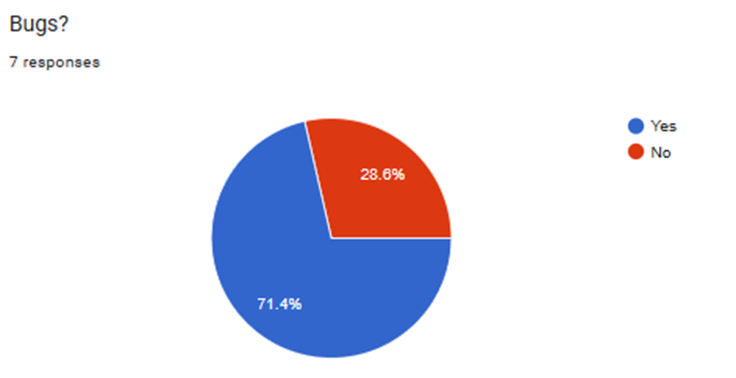
\includegraphics[width=1\textwidth]{figures/Bug1.png}
    \caption{Survey for Bugs}
    \label{fig:bug_survey}
    \end{minipage}
    \hfill
    \begin{minipage}{0.49\textwidth}
    \centering
    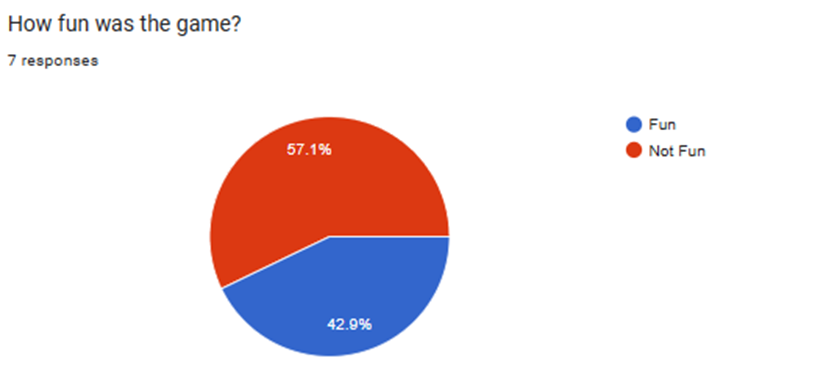
\includegraphics[width=1\textwidth]{figures/Fun1.png}
    \caption{Players Experience}
    \label{fig:player_experience}
    \end{minipage}
\end{figure}



\noindent These initial survey results highlighted the need for immediate attention and improvement in various aspects of the game, including bug fixing, gameplay mechanics refinement, and overall user experience enhancement.

\section{Post-Improvement Survey Results}
After implementing significant improvements and refinements based on the feedback from the initial survey, a second survey was conducted to assess the impact of the changes. The results were remarkably positive, validating the effectiveness of the development efforts.
\\

\begin{figure}[h]
    \centering
    \begin{minipage}{0.49\textwidth}
    \centering
    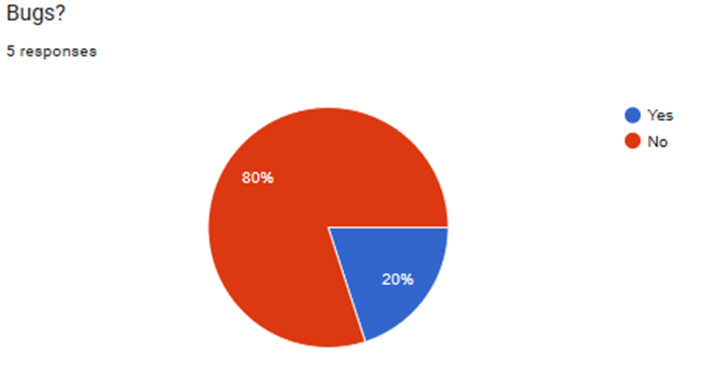
\includegraphics[width=1\textwidth]{figures/Bug2.png}
    \caption{Survey for Bugs}
    \label{fig:bug_survey1}
    \end{minipage}
    \hfill
    \begin{minipage}{0.49\textwidth}
    \centering
    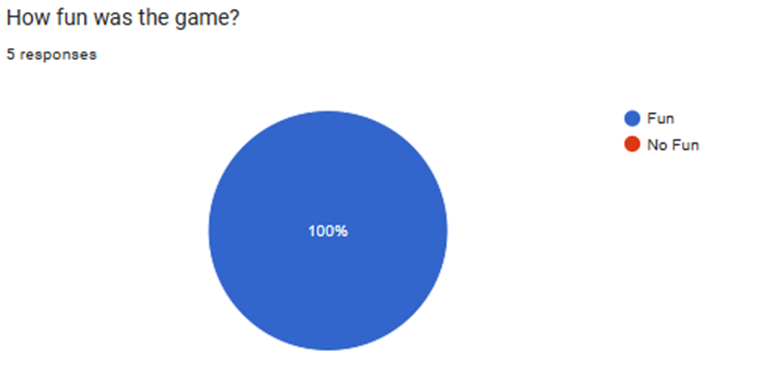
\includegraphics[width=1\textwidth]{figures/Fun2.png}
    \caption{Players Experience}
    \label{fig:player_experience1}
    \end{minipage}
\end{figure}

\noindent An astounding 100\% of the participants found the game to be fun and engaging, a testament to the successful enhancements made to the gameplay mechanics and overall experience. Moreover, 80\% of the participants reported a significant reduction in bugs, indicating that the extensive testing and optimisation efforts had paid off.
\\
\noindent
\\
These survey results demonstrate the project's ability to address and overcome the initial challenges, ultimately delivering an engaging and accessible online multiplayer tank battle game.

\section{Summary}
This chapter presented the results achieved through the development and implementation of Tank Tactics, showcasing the successful integration of seamless multiplayer connectivity, engaging gameplay mechanics, and advanced features. The survey results and player feedback provided valuable insights into the game's performance and user experience, highlighting areas for improvement and validating the effectiveness of the implemented enhancements.
\\
\noindent
\\
The positive outcomes and survey results demonstrate the project's success in achieving its primary objectives, as outlined in Chapter 1, and addressing the challenges associated with traditional online multiplayer games, as discussed in Chapter 2.



